\section{Standard momentum descent (heavy ball)}
In this section we will talk about the fourth and last method considered for solving the lls problem, we will proceed as we did for the L-BFGS, thin QR and conjugate gradient.

\subsection{Overview on gradient descent}
Gradient descent is the most well-known way to minimize an objective function $J(W)$ parameterized by a model's parameters $W \in \mathbb{R}^d$ by updating such parameters in the opposite direction of the gradient of the objective function $\nabla_{W}J(W)$  w.r.t. to the parameters. The learning rate $\eta$ determines the size of the steps we take to reach a (local) minimum. In other words, we follow the direction of the slope of the surface created by the objective function downhill until we reach a valley.
\vspace{3mm}

\noindent Let's take a look at the easiest implementation that computes the gradient of the cost function w.r.t. to the parameters $W$ for the entire training dataset (the so called batch version).
\begin{equation}
    W = W - \eta \nabla J(W)
    \label{eq:smd_batch_gradient_descent}
\end{equation}
The main issue of such method is the slow convergence, resulting in an extremely high number of iterations. To alleviate this behavior the momentum descend approach can be used.

\subsection{Standard momentum descent}
\iffalse
The momentum algorithm allows to accelerate the gradient descent as in the detected direction it adds a fraction $\beta$ of the vector calculated in the previous step to the current update vector. The similarity of this approach is to drop a heavy ball from a cliff, the latter will begin to descend accumulating momentum and rolling faster resulting in better stability. The same thing happens to weight updates, the momentum variable boosts gradients pointing to the same descent direction and reduces updates on gradients pointing to different directions. As a result we have the fastest convergence, the reduction of oscillations and the possibility of using a higher learning rate.
\begin{figure}[H]
    \centering
    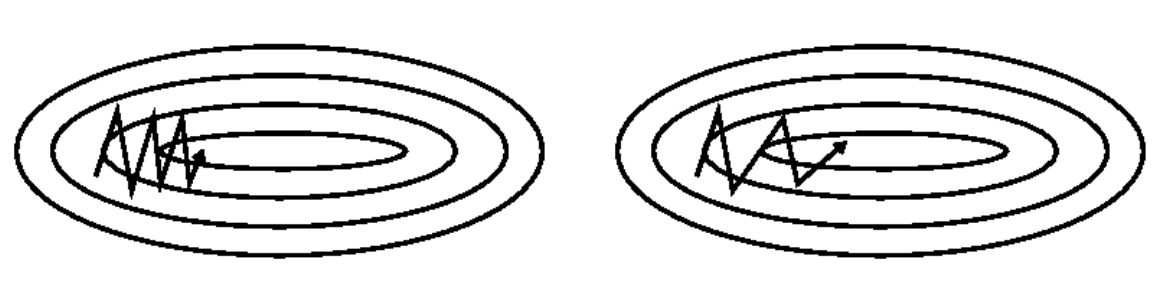
\includegraphics[width=0.5\linewidth]{images/smd/momentum.PNG}
    \caption{Left — SGD without momentum, right— SGD with momentum.}
    \label{fig:smd_momentum}
\end{figure}
\fi

\noindent The standard momentum descent is a technique first presented by Polyak \cite{POLYAK19641} that introduces a variable $V$ which accumulates the velocity towards directions of persisted reduction in the objective across iterates \cite{pmlr-v28-sutskever13}. The momentum algorithm allows to accelerate the gradient descent as in the detected direction it adds a fraction $\beta$ of the vector calculated in the previous step to the current update vector. The hyper-parameters are the learning rate $\eta$ and the momentum $\beta \in [0,1)$, the latter typically chosen as 0.9. If $\beta = 0$, then classical momentum reduces to the gradient method. The parameters update works as follow: 
\begin{subequations}
    \begin{equation}
        V_{dw} = \beta V_{dw} - \eta*dW
    \end{equation}
    \begin{equation}
        W = W + V_{dw}
    \end{equation}
    \label{eq:momentum_descent}
\end{subequations}

\subsection{Solving LLS with standard momentum descent}
The idea behind gradient descent is pretty similar to the one seen for conjugate gradient. Gradient descent can be used to solve a system of linear equation $Ax - b = 0$, where $A$ is symmetric and positive definite, but, as we know, the $\hat{X}$ matrix has not the same proprieties of $A$, so in order to apply gradient descent to our problem we need to define $A = \hat{X}^T \hat{X}$ and $b = \hat{X}^T \hat{y}$. We have already explained this fact when we described how to solve LLS problem while using conjugate gradient in \ref{subsec:solve_LLS_cg}. For this reason, we will not talk again about the preliminary part to do before starting to apply the algorithm.
\vspace{3mm}

\noindent The gradient descent algorithm differs a bit from the conjugate gradient one, so we are going to report it. Also, even for this algorithm, we do not explicitly compute the matrix $A$, even if it would have saved us time, because we preferred to get more qualitative results by limiting the condition number of $A$.

\begin{algorithm}[H]
    \caption{Standard momentum descent}
    \label{algorithm:smd_lls}
    Given $w_0 \in R^m$, $\beta$, $v = 0$;\\
    \While{$k<max\_iterations$ and $error \geq tol$} {
        $r_k=b-Aw_k$;\\
        $\eta = \frac{r_{k}^{T} r_{k}}{r_{k}^{T} A r_{k}}$;\\
        $v = \beta v + \eta r_k$;\\
        $w_k = w_k + v$;\\
        $k=k+1$;\\
    }
    \Return{$w$};
\end{algorithm}

\noindent The computational cost of gradient descent is dominated by matrix-vector products and fortunately, one can be eliminated. If we do not consider the momentum update rule, we get $w = w + \eta r_k$ and by premultiplying both sides of this equation by $-A$ and adding b, we have that
\begin{equation}
    r_k = r_k - \eta A r_k
    \label{eq:smd_rk}
\end{equation}
so we can store the result of $A r_k$ in order to avoid to compute it twice per iteration. The starting point for $r$ still remains $r_0 = b - A w_0$, then it gets updated by using the new formula. The disadvantage of using this recurrence is that the sequence defined by \eqref{eq:smd_rk} is generated without any feedback from the value of $w_i$, so that accumulation of floating point round-off error may cause $w_i$ to converge to some point near $w$. This effect can be avoided by periodically using $r_k=b-Aw_k$ to recompute the correct residual as suggested by Shewchuk et al. \cite{shewchuk1994introduction}.

\subsection{Convergence analysis with exact line search}\label{subsec:smd_convergence}
Assume that $f$ is strongly convex on $S$, so there are positive constants $\theta_1$ and $\theta_n$ such that $\theta_1I \leq \nabla^{2}f(x) \leq \theta_nI, \forall x \in S$. By using the lighter notation $x^{(k+1)} = x^{(k)} + \eta^{(k)}\Delta x^{(k)}$, Boyd and Vandenberghe \cite{boyd2004convex} state that
\begin{equation}
    f(x^{(k)}) - p^{*} \leq c^{k}(f(x^{(0)}) - p^{*})
    \label{eq:conv_grad_descent}
\end{equation}
where $p^*$ is the optimal value of the function $f$ and $c = 1 - \theta_1/\theta_n < 1$ \footnote{recalling that $\kappa = \theta_n/\theta_1 $ is an upper bound on the condition number of the matrix $\nabla^2f(x)$, \textit{i.e.} the ratio of its largest eigenvalue to its smallest eigenvalue.}, which shows that $f(x^{(k)})$ converges to $p^*$ as $k \rightarrow \infty$. In particular, we must have $f(x^{(k)}) - p^* \leq \epsilon$ after at most 
\begin{equation}
    \frac{log((f(x^{(0)})-p^*)/\epsilon)}{log(1/c)}
    \label{eq:iter_grad_descent}
\end{equation}
iterations of the gradient method with exact line search. We can now analyze what kind of information can be derived from both the numerator and the denominator. The first one can be interpreted as the log of the ratio of the initial sub-optimality (\textit{i.e.}, gap between $f(x^{0})$ and $p^*$, to the final sub-optimality (\textit{i.e.} less than $\epsilon$). This term
suggests that the number of iterations depends on how good the initial point is, and what the final required accuracy is. Instead, the denominator of \eqref{eq:iter_grad_descent} is a function of $\theta_n/\theta_1$, which we have seen is a bound on the condition number of $\nabla^2 f(x)$ and for large condition number bound $\theta_n/\theta_1$, we have 
\begin{equation}
    log(1/c) = -log(1-\theta_1/\theta_n) \approx \theta_1/\theta_n
\end{equation}
meaning that our bound on the number of iterations required increases approximately linearly following the increasing of $\theta_n/\theta_1$. This fact lead the gradient method to require a large number of iterations when the Hessian of $f$, near $x^*$, has a large condition number. Finally, the bound \eqref{eq:conv_grad_descent} shows that the error $f(x^{(k)}) - p^{*}$ converges to zero at least as fast as a geometric series that, in the context of iterative numerical methods, is called linear convergence.

\subsection{Convergence analysis of heavy ball}
\label{subsec:hbm_convergence}
Again, we know that $f$ is strongly convex on $S$, so there are positive constants $\theta_1$ and $\theta_n$ such that $\theta_1I \leq \nabla^{2}f(x) \leq \theta_nI, \forall x \in S$. The heavy ball method adds a momentum term in gradient descent:
\begin{equation}
    x_{k+1} = x_{k} - \eta_{k} \nabla_{x} f(x_k) + \underbrace{\beta_k (x_k - x_{k-1})}_{\text{HBM  momentum}}
    \label{eq:hb_update_xk}
\end{equation}

\noindent Consider $x_{k+1} - x^*$. By definition of HBM update \eqref{eq:hb_update_xk}, 
\begin{equation}
    x_{k+1} - x^* = x_{k} - \eta_{k} \nabla_{x} f(x_k) + \beta_k (x_k - x_{k-1}) - x^*
    \label{eq:hb_update_xk_2}
\end{equation}

\noindent As $\nabla_x f(x_k) = Ax_k - b$ and $b = Ax^*$, we have $\nabla_x f(x_k) = Ax_k - Ax^*$. By developing \eqref{eq:hb_update_xk_2}, we have:
\begin{equation}
\begin{aligned}
x_{k+1} - x^* &= x_k - x^* - \eta_k A(x_k - x^*) + \beta(x_k - x_{k-1}) \\
& = (I - \eta_k A)(x_k - x^*) + \beta_k (x_k - x_{k-1} -x^* + x^*) \\
& = (I - \eta_k A)(x_k - x^*) - \beta_k (x_{k-1} - x^*) + \beta(x_k - x^*)\\
&= \left((1+\beta_k)I-\eta_k A)\right(x_k - x^*) - \beta_k (x_{k-1} - x^*)
\end{aligned}
\end{equation}

\noindent In this sense, we have to consider $x_k - x^*$ and $x_{k-1} - x^* $ at the same time
\begin{equation}
\begin{bmatrix}
x_{k+1} - x^*\\
x_k - x^*
\end{bmatrix} 
=
\underbrace{\begin{bmatrix}
(1+\beta_k)I - \eta_k A & - \beta_kI\\
I & 0
\end{bmatrix}}_{T_k (\eta, \beta)}
\begin{bmatrix}
x_{k} - x^*\\
x_{k-1} - x^*
\end{bmatrix}
\end{equation}
where $T_k (\eta, \beta)$ is the transition matrix. For simplicity we consider the compact expression

\begin{equation}
\begin{bmatrix}
x_{k+1} - x^*\\
x_k - x^*
\end{bmatrix} 
=
T_k(\eta, \beta)
\begin{bmatrix}
x_{k} - x^*\\
x_{k-1} - x^*
\end{bmatrix}
\end{equation}
Take constant $\eta_k$ and $\beta_k$ in $T_k$, so $T_k = T$ and 

\begin{equation}
\begin{bmatrix}
x_{k+1} - x^*\\
x_k - x^*
\end{bmatrix} 
=
T^k
\begin{bmatrix}
x_{1} - x^*\\
x_{0} - x^*
\end{bmatrix}
\end{equation}
Take the norm

\begin{equation}
\left\lVert
\begin{bmatrix}
x_{k+1} - x^*\\
x_k - x^*
\end{bmatrix}
\right\rVert
=
\left\lVert
T^k
\begin{bmatrix}
x_{1} - x^*\\
x_{0} - x^*
\end{bmatrix}
\right\rVert
\leq
\lVert
T^k
\rVert
\left\lVert
\begin{bmatrix}
x_{1} - x^*\\
x_{0} - x^*
\end{bmatrix}
\right\rVert
\end{equation}
So, if $\lVert T^k \rVert$ is bounded, the series $x_k$ produced by the heavy ball method converges. In order to explain this we need two lemmas, for which we omit the proof.

\begin{lemma}
For a matrix $T \in \mathbb{R}^{n\times n}$, there exists a sequences $\epsilon_k \geq 0$ such that $\lVert T^k \rVert \leq (\rho(T) + \epsilon_k)^k$ where $\displaystyle \lim_{k \rightarrow \infty}{\epsilon_k = 0} $.
\label[lemma]{le:lemma1}
\end{lemma}

\begin{lemma}
For $\beta>(1 - \sqrt{\eta \theta_n})^2$, $\rho(T) < \beta$, where $\rho(T) = \max{\{|\psi_1|, |\psi_2|, \dots, |\psi_n|\}}$ is the spectral radius of matrix $T$ and $\psi_i$ are the eigenvalues of $T$.
%\label{le:lemma2}
\label[lemma]{le:lemma2}
\end{lemma}

\noindent Now, assume $\beta>(1 - \sqrt{\eta \theta_n})$, by \cref{le:lemma2} we have $\rho(T) = \max{|\psi_i(T)|} \leq \beta$. By \cref{le:lemma1}, we have $\lVert T^k \rVert \leq (\rho(T) + \epsilon_k)^k$ with $\displaystyle \lim_{k \rightarrow \infty}{\epsilon_k = 0}$. Putting \cref{le:lemma2} into \cref{le:lemma1} we obtain:
\begin{equation}
    \lVert T^k \rVert \leq (\beta + \epsilon_k)^k
\end{equation}

\vspace{3mm}

\noindent Lastly, let $\eta = \frac{4}{(\sqrt{\theta_n}+\sqrt{\theta_1})^2}$ and $\beta = \frac{\sqrt{\theta_n} - \sqrt{\theta_1}}{\sqrt{\theta_n}+\sqrt{\theta_1}}$ in $T$ we have:
\begin{equation}
\left\lVert
\begin{bmatrix}
x_{k+1} - x^*\\
x_k - x^*
\end{bmatrix}
\right \rVert
\leq \left(\frac{\sqrt{\theta_n} - \sqrt{\theta_1}}{\sqrt{\theta_n}+\sqrt{\theta_1}} + \epsilon \right)^k
\left\lVert
\begin{bmatrix}
x_{1} - x^*\\
x_{0} - x^*
\end{bmatrix}
\right\rVert
\end{equation}
or:
\begin{equation}
    \lVert x_k - x^* \rVert \leq \left(\frac{\sqrt{\kappa} - 1}{\sqrt{\kappa}+1} + \epsilon \right)^k \lVert x_0 - x^* \rVert
\end{equation}
 where $\kappa = \frac{\theta_n}{\theta_1}$. By exploiting momentum, we benefit of an improvement from $ \left(\frac{\kappa - 1}{\kappa + 1} + \epsilon \right)^k$ of the standard gradient descent to $\left(\frac{\sqrt{\kappa} - 1}{\sqrt{\kappa}+1} + \epsilon \right)^k$ of the heavy ball method. This result is similar to the one obtained for the conjugate gradient method, in \eqref{eq:cg_rewritten_epsilon}.

\subsection{Performance analysis}

\subsubsection{Linear rate of convergence}
In \ref{subsec:hbm_convergence}, we stated that the standard momentum descent algorithm has a linear convergence rate due to the fact that our function is strongly convex.
\vspace{3mm}

\noindent In \autoref{fig:convergence_smd} we can empirically confirm that our implementation has the theoretically expected convergence rate. Moreover we can notice that when $\hat{X}^T\hat{X}$ becomes more and more ill-conditioned, the GD method requires more steps to converge, as discussed in \ref{subsec:smd_convergence}.

\begin{figure}[H]
    \centering
    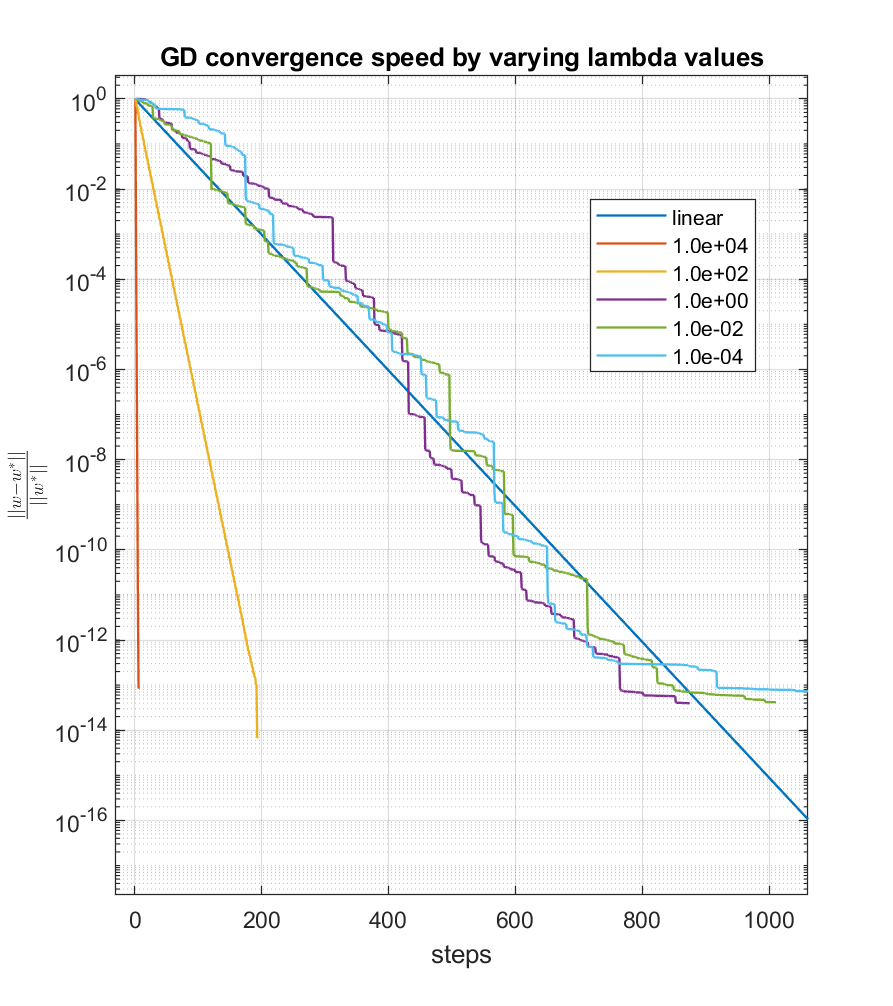
\includegraphics[width = 0.7\linewidth]{images/smd/momentum_comparison_smd_linear_fixed.png}
    \caption{GD convergence speed by varying lambdas values, with momentum.}
    \label{fig:convergence_smd}
\end{figure}

\subsubsection{Effect of momentum}
A fundamental analysis involves the role of $\beta$ in our method, therefore,
in order to find the best value for such hyper-parameter, we ran a grid search. For instance, in \autoref{fig:smd_comparing_betas}, we fixed the problem (same input matrix, expected values and starting point) and we found that the best value for $\beta$ was equal to $0.05$, of course, this value can greatly differ from problem to problem. In our case, a too high momentum slows down the convergence speed, increasing the total amount of steps needed to reach the convergence.

\begin{figure}[H]
    \centering
    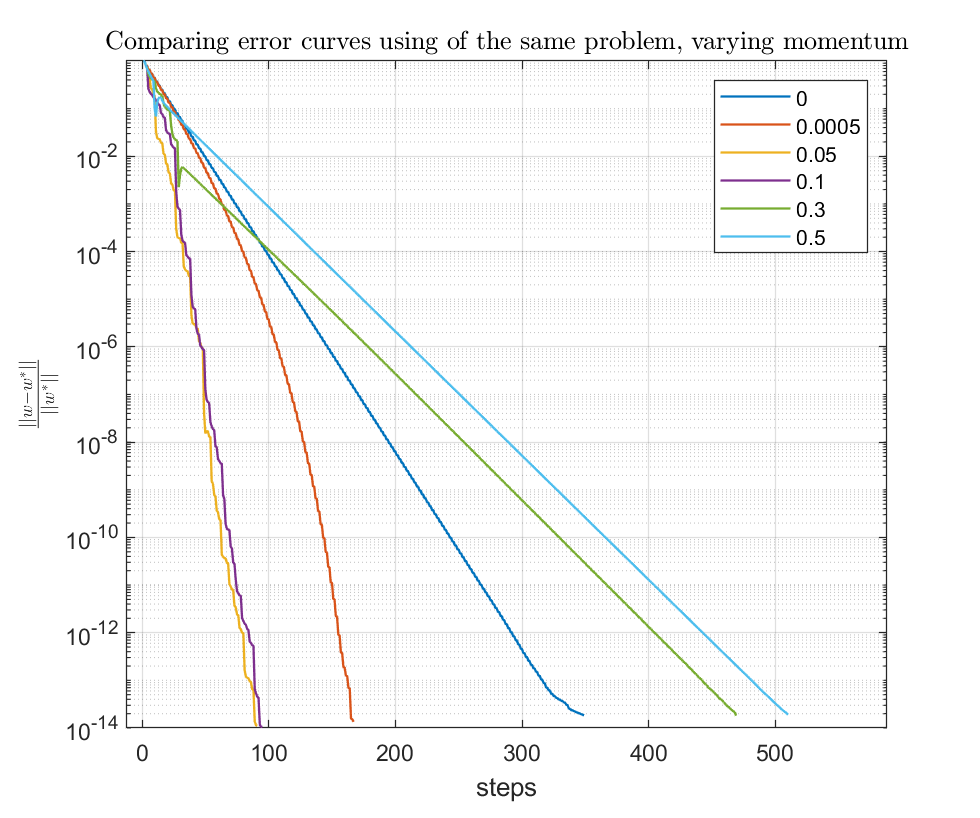
\includegraphics[width = 0.8\linewidth]{images/smd/momentum_comparison_smd.png}
    \caption{GD convergence speed by varying $\beta$ values.}
    \label{fig:smd_comparing_betas}
\end{figure}

\noindent It is interesting to notice that the introduction of momentum makes our method faster, when chosen appropriately, but, on the other side, we can say that it becomes more unstable by looking at \autoref{fig:smd_comparing_betas}.

\paragraph{Side by side comparison}
We will now graphically view the effect of momentum in reducing the total amount of steps required by the gradient descent to converge. In \autoref{fig:smd_with_without_momentum} it is clearly visible that momentum plays an important role, in fact it allowed us to reduce the total amount of steps to reach the convergence especially when the Hessian becomes ill-conditioned.

\begin{figure}[H]
    \centering
    \subfloat[Gradient descent with momentum]{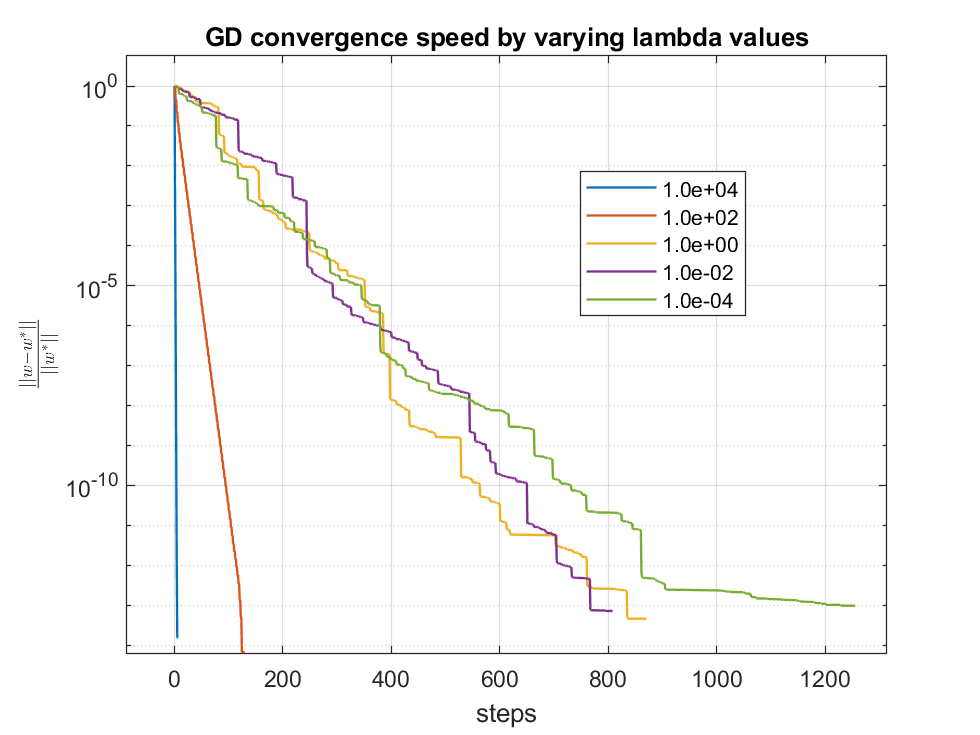
\includegraphics[width=0.52\linewidth]{images/smd/smd_comparison_with_momentum.png}}
    \subfloat[Gradient descent without applying momentum]{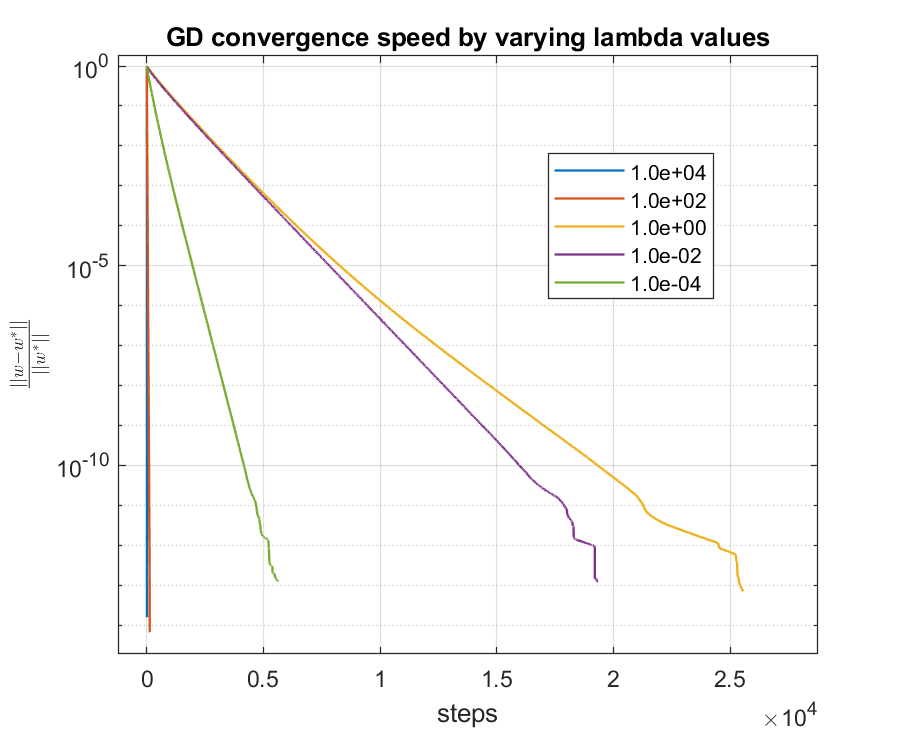
\includegraphics[width=0.48\linewidth]{images/smd/smd_comparison_no_momentum.png}}
    \caption{Side by side comparison between the steps necessary to converge by GD method, with and without momentum.}
    \label{fig:smd_with_without_momentum}
\end{figure}

\subsubsection{Results}
By looking at \autoref{tab:smd_results}, it is possible to notice that the relative errors and the relative residuals are pretty similar to the conjugate gradient ones from \autoref{tab:cg_results}, since the two methods are related. Furthermore, in terms of relative error and amount of steps to reach the convergence, the algorithm performed better without using momentum only for $\lambda = 10^4$, whereas, in the remaining cases we tested, adding momentum allowed us to reach the solution in a faster way as already seen from \autoref{fig:smd_with_without_momentum}. As usual, $w^*$ is the Matlab solution $\hat{X}\backslash \hat{y}$ and, from \ref{subsec:introduction_convexity}, such minima is unique and global.

\begin{table}[H]
\small
\centering
\begin{tabular}{c|c|c|c|c|c} \hline \hline
    $\lambda$& $\beta$ &$\frac{\lVert w - w^{*} \lVert}{\rVert w^{*} \lVert}$ & $\frac{\lVert \hat{X}w - y \lVert }{\lVert y \lVert}$ & steps & time (sec)\\ \hline \hline
    
    \rowcolor{gray!30} $10^4$ & $0$ & $ 3.49 \times 10^{-14} \pm 2.15 \times 10^{-14}$ &$9.99 \times 10^{-1} \pm 3.04 \times 10^{-4}$ & $19 \pm 9$& $9.56 \times 10^{-4}$ \\
    
    $10^2$ & $ 0.05$ & $ 8.67 \times 10^{-15} \pm 8.08 \times 10^{-16}$ &$9.39 \times 10^{-1} \pm 4.21 \times 10^{-2}$&$106 \pm 10$& $4.12 \times 10^{-3}$ \\
    
    \rowcolor{gray!30} $1$ & $0.05$ & $ 3.51 \times 10^{-14} \pm 1.85 \times 10^{-14} $ &$ 5.61 \times 10^{-2} \pm 5.66 \times 10^{-3} $&$1350 \pm 342$& $4.91 \times 10^{-2}$ \\
    
    $10^{-2}$ & $ 0.05$ & $5.77 \times 10^{-14} \pm 3.08 \times 10^{-14}$ & $5.07 \times 10^{-4} \pm 7.58 \times 10^{-5}$&$1075 \pm 78$& $3.84 \times 10^{-2}$ \\
    
    \rowcolor{gray!30} $10^{-4}$ & $0.05$ & $6.42 \times 10^{-14} \pm 2.57 \times 10^{-14}$ &$5.42 \times 10^{-6} \pm 8.26 \times 10^{-7}$&$1148 \pm 59$ & $4.10 \times 10^{-2}$ \\
    \hline \hline
\end{tabular}
\caption{Standard momentum descent results.}
\label{tab:smd_results}
\end{table}
